
\subsection{The simplicity of \texorpdfstring{$\sl(2,\C)$}{sl(2,C)}}
We have seen that the non-zero structure constants of $T_{\left(\begin{smallmatrix}1 & 0 \\ 0 & 1\end{smallmatrix}\right)}\SL(2,\C)$ are
\bse
C^2_{\phantom{2}12} = 2, \qquad C^3_{\phantom{3}13}=-2,\qquad C^1_{\phantom{1}23}=1,
\ese
plus those related by anti-symmetry. 
\bp
Two Lie algebras $A$ and $B$ are isomorphic if, and only if, there exists a basis of $A$ and a basis of $B$ in which the structure constants of $A$ and $B$ are the same.
\ep
Since we have already proved that $T_eG\cong_{\mathrm{Lie \, alg}}\mathcal{L}(G)$ for any Lie group $G$, we can deduce the existence of a basis $\{X_1,X_2,X_2\}$ of $\sl(2,\C)$ with respect to which the structure constants are those listed above. In other words, we have
\bi{rCl}
[X_1,X_2] & = & 2X_2,\\
{[X_1,X_3]} & = & -2X_3,\\
{[X_2,X_3]} & = & X_1.
\ei
In this basis, the Killing form of $\sl(2,\C)$ has components
\bse
\kappa_{ij} = C^{m}_{\phantom{m}in}C^{n}_{\phantom{n}jm},
\ese
with all indices ranging from $1$ to $3$. Explicitly, we have
\bi{rCl}
\kappa_{11} & = & C^{m}_{\phantom{m}1n}C^{n}_{\phantom{n}1m}\\
 & = & \Ccancel[gray]{C^{1}_{\phantom{1}1n}C^{n}_{\phantom{n}11}} + C^{2}_{\phantom{2}1n}C^{n}_{\phantom{n}12} + C^{3}_{\phantom{3}1n}C^{n}_{\phantom{n}13}\\
 & = & C^{2}_{\phantom{2}12}C^{2}_{\phantom{2}12} + C^{3}_{\phantom{3}13}C^{3}_{\phantom{3}13}\\
 & = & 8.
\ei
Since $\kappa$ is symmetric, we only need to determine $\kappa_{ij}$ for $i\leq j$. By writing the components in a $3\times 3$ array, we find
\bse
[\kappa_{ij}] = \left(\begin{matrix}8 & 0 & 0 \\ 0 & -8 & 0 \\ 0 & 0 & 8\end{matrix}\right),
\ese
which is just shorthand for 
\bse
\kappa(X_1,X_1) = 8, \qquad 
\kappa(X_2,X_2) = -8, \qquad 
\kappa(X_3,X_3) = 8,
\ese
and $\kappa(X_i,X_j)=0$ whenever $i\neq j$.

\bp
The Lie algebra $\sl(2,\C)$ is semi-simple.
\ep

\bq
Since the diagonal entries of $\kappa$ are all non-zero, the Killing form is non-degenerate. By Cartan's criterion, this implies that $\sl(2,\C)$ is semi-simple.
\eq

\br
There is one more thing that can be read off from the components of $\kappa$, namely, that it is an \emph{indefinite} form, i.e.\ the sign of $\kappa(X,X)$ can be positive or negative depending on which $X\in \sl(2,\C)$ we pick.

A result from Lie theory states that the Killing form on the Lie algebra of a compact Lie group is always negative semi-definite, i.e.\ $\kappa(X,X)$ is always negative or zero, for all $X$ in the Lie algebra. Hence, we can conclude that $\SL(2,\C)$ is not a compact Lie group.
\er
In fact, $\sl(2,\C)$ is more than just semi-simple.

\bp
The Lie algebra $\sl(2,\C)$ is simple.
\ep
Recall that a Lie algebra is said to be simple if it contains no non-trivial ideals, and that an ideal $I$ of a Lie algebra $L$ is a Lie subalgebra of $L$ such that
\bse
\forall \, x \in I : \forall \, y\in L : \ [x,y] \in I.
\ese

\bq
Consider the ideal of $\sl(2,\C)$
\bse
I := \{\alpha X_1+\beta X_2 + \gamma X_3 \mid \alpha,\beta,\gamma \text{ restricted so that $I$ is an ideal}\}.
\ese
Since the bracket is bilinear, it suffices to check the result of bracketing an arbitrary element of $I$ with each of the basis vectors of $\sl(2,\C)$. We find
\bi{rCl}
[\alpha X_1+\beta X_2 + \gamma X_3,X_1] & = & -2\beta X_1+2\gamma X_3,\\[2pt]
{[\alpha X_1+\beta X_2 + \gamma X_3,X_2]} & = & 2 \alpha X_2 - \gamma X_1,\\[2pt]
{[\alpha X_1+\beta X_2 + \gamma X_3,X_3]} & = & -2\alpha X_3 +\beta X_1.
\ei
We need to choose $\alpha,\beta,\gamma$ so that the results always land back in $I$. Of course, we can choose $\alpha,\beta,\gamma\in\C$ and $\alpha=\beta=\gamma=0$, which correspond respectively to the trivial ideals $\sl(2,\C)$ and $0$. If none of $\alpha,\beta,\gamma$ is zero, then you can check that the right hand sides above are linearly independent, so that $I$ contains three linearly independent vectors. Since the only $n$-dimensional subspace of an $n$-dimensional vector space is the vector space itself, we have $I=L$. Thus, we are left with the following cases:
\ben[label=\roman*)]
\item if $\alpha = 0$, then $I\se \lspan_\C(\{X_2,X_3\})$ and hence we must have $\beta = \gamma = 0$ as well;
\item if $\beta = 0$, then $I\se \lspan_\C(\{X_1,X_3\})$, hence we must have $\alpha = 0$, so that in fact $I\se \lspan_\C(\{X_3\})$, and hence $\gamma = 0$ as well;
\item if $\gamma = 0$, then $I\se \lspan_\C(\{X_1,X_2\})$, hence we must have $\alpha = 0$, so that in fact $I\se \lspan_\C(\{X_2\})$, and hence $\beta = 0$ as well.
\een
In all cases, we have $I=0$. Therefore, there are no non-trivial ideals of $\sl(2,\C)$.
\eq

\subsection{The roots and Dynkin diagram of \texorpdfstring{$\sl(2,\C)$}{sl(2,C)}}

By observing the bracket relations of the basis elements of $\sl(2,\C)$, we can see that
\bse
H:=\lspan_\C(\{X_1\})
\ese
is a Cartan subalgebra of $\sl(2,\C)$. Indeed, for any $h\in H$, there exists a $\xi \in \C$ such that $h=\xi X_1$, and hence we have
\bi{rCl}
\ad(h) X_2 & = & \xi [X_1,X_2] = 2\xi X_2,\\
\ad(h) X_3 & = & \xi [X_1,X_3] = -2\xi X_3.
\ei
Recall that in the section on Lie algebras, we re-interpreted these eigenvalue equations in terms of functionals $\lambda_2,\lambda_3\in H^*$ 
\bi{rrClrrCl}
\lambda_2\cl & H & \xrightarrow{\sim} & \C \qquad \qquad & \lambda_3\cl & H & \xrightarrow{\sim} & \C\\
& \xi X_1 & \mapsto & 2\xi, & & \xi X_1 & \mapsto & -2\xi 
\ei
whereby
\bi{rCl}
\ad(h) X_2 & = &\lambda_2(h) X_2,\\
\ad(h) X_3 & = & \lambda_3(h) X_3.
\ei
Then, $\lambda_2$ and $\lambda_3$ are called the roots of $\sl(2,\C)$, so that the root set is $\Phi=\{\lambda_2,\lambda_3\}$. Of course, we are mainly interested in a subset $\Pi\ss \Phi$ of fundamental roots, which satisfies
\ben[label=\roman*)]
\item $\Pi$ is a linearly independent subset of $H^*$;
\item for any $\lambda\in \Phi$, we have $\lambda \in \lspan_{\epsilon,\N}(\Pi)$.
\een
We can choose $\Pi:=\{\lambda_2\}$, even though $\Pi:=\{\lambda_3\}$ would work just as well. Since $|\Pi|=1$, the Weyl group is generated by the single Weyl transformation
\bi{rrCl}
s_{\lambda_2}\cl & H^*_\R & \to & H^*_\R\\
& \mu & \mapsto & \mu - 2\frac{\kappa^*(\lambda_2,\mu)}{\kappa^*(\lambda_2,\lambda_2)}\lambda_2 .
\ei
Recall that we can recover the entire root set $\Phi$ by acting on the fundamental roots with Weyl transformations. Indeed, we have
\bse
s_{\lambda_2}(\lambda_2) = \lambda_2- 2\frac{\kappa^*(\lambda_2,\lambda_2)}{\kappa^*(\lambda_2,\lambda_2)}\lambda_2 = \lambda_2-2\lambda_2 = -\lambda_2 = \lambda_3,
\ese
as expected. Since there is only one fundamental root, the Cartan matrix is actually just a $1\times 1$ matrix. Its only entry is a diagonal entry, and since $\sl(2,\C)$ is simple,
 we have
\bse
C = (2). 
\ese
The Dynkin diagram of $\sl(2,\C)$ is simply 
\begin{center}
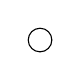
\begin{tikzpicture}
\draw[fill=white] (0,0) circle[radius=0.15];
\end{tikzpicture}
\end{center}
Hence, with reference to the Cartan classification, we have $A_1 = \sl(2,\C)$.

\subsection{Reconstruction of \texorpdfstring{$A_2$}{A2} from its Dynkin diagram}

We have seen an example of how to construct the Dynkin diagram of a Lie algebra, albeit the simplest of this kind. Let us now consider the opposite direction. We will start from the  Dynkin diagram
\begin{center}
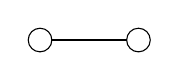
\begin{tikzpicture}
\draw (0,0) -- (1.25,0);
\draw[fill=white] (0,0) circle[radius=0.15];
\draw[fill=white] (1.25,0) circle[radius=0.15];
\end{tikzpicture}
\end{center}
We immediately see that we have two fundamental roots, i.e.\ $\Pi = \{\pi_1,\pi_2\}$, since there are two circles in the diagram. The bond number is $n_{12} = 1$, so the two fundamental roots have the same length. Moreover, by definition
\bse
1=n_{12} = C_{12}C_{21}
\ese
and since the off-diagonal entries of the Cartan matrix are non-positive integers, the only possibility is $C_{12}=C_{21}=-1$, so that we have
\bse
C = \biggl( \begin{matrix}2 & -1\\ -1 & 2\end{matrix}\biggr).
\ese
To determine the angle $\varphi$ between $\pi_1$ and $\pi_2$, recall that
\bse
1 = n_{12} = 4 \cos^2\varphi,
\ese
and hence $|\cos\varphi|=\frac{1}{2}$. There are two solutions, namely $\varphi=60^\circ$ and $\varphi=120^\circ$.
\begin{center}
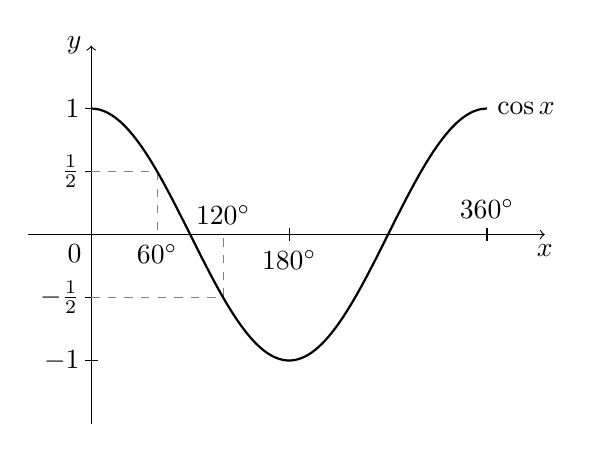
\begin{tikzpicture}[xscale=0.8,yscale=1.6]
\draw[->] (-1,0) -- (7.2,0) node[below] {$x$};
\draw[->] (0,-1.5) -- (0,1.5) node[left] {$y$};
\foreach \i/\j in {-2/-1,-1/-\frac{1}{2},1/\frac{1}{2},2/1} {
\draw (-0.1,0.5*\i) -- (0.1,0.5*\i) node[left=3pt] {$\j$};
}
\draw (0,0) node[below left] {$0$};
\draw[gray,dashed] (0,0.5) -| (pi/3,0);
\draw (pi/3,0) node[below] {$60^\circ$};
\draw[gray,dashed] (0,-0.5) -| (2*pi/3,0);
\draw (2*pi/3,0) node[above] {$120^\circ$};
\draw (pi,0.05) -- (pi,-0.05) node[below] {$180^\circ$};
\draw (2*pi,-0.05) -- (2*pi,0.05) node[above] {$360^\circ$};
\draw[thick,smooth,samples=100,variable=\x,domain=0:2*pi] plot(\x,{cos(deg(\x))}) node[right] {$\cos x$};
\end{tikzpicture}
\end{center}
By definition, we have
\bse
\cos \varphi = \frac{\kappa^*(\pi_1,\pi_2)}{|\pi_1|\,|\pi_2|},
\ese
and therefore
\bse
0 > C_{12} = 2\frac{\kappa^*(\pi_1,\pi_2)}{\kappa^*(\pi_1,\pi_1)} = 2\frac{|\pi_1|\,|\pi_2|\cos\varphi}{\kappa^*(\pi_1,\pi_1)} = 2\frac{|\pi_2|}{|\pi_1|}\cos\varphi.
\ese
It follows that $\cos\varphi<0$, and hence $\varphi = 120^\circ$. We can thus plot the two fundamental roots in a plane as follows.
\begin{center}
\begin{tikzpicture}[scale=2]
\draw[thin,lightgray] (-1.5,0) -- (1.5,0);
\draw[thin,lightgray] (0,-1.25) -- (0,1.25);
\draw[thick,->] (0,0) -- (1,0) node[above right] {$\pi_1$};
\draw[thick,->] (0,0) -- (cos 120,sin 120) node[above left] {$\pi_2$};
\end{tikzpicture}
\end{center}
We can determine all the other roots in $\Phi$ by repeated action of the Weyl group. For instance, we easily find that $s_{\pi_1}(\pi_1) = -\pi_1$ and $s_{\pi_2}(\pi_2) = -\pi_2$. We also have
\bse
s_{\pi_1}(\pi_2)  =  \pi_2-2\frac{\kappa^*(\pi_1,\pi_2)}{\kappa^*(\pi_1,\pi_1)}\pi_1 = \pi_2 -2 (-\tfrac{1}{2}) \pi_1 = \pi_1+\pi_2.
\ese
Finally, we have $s_{\pi_1+\pi_2}(\pi_1+\pi_2)=-(\pi_1+\pi_2)$.  Any further action by Weyl transformations simply permutes these roots. Hence, we have
\bse
\Phi=\{\pi_1,-\pi_1,\pi_2,-\pi_2,\pi_1+\pi_2,-(\pi_1+\pi_2)\}
\ese
and these are all the roots.
\begin{center}
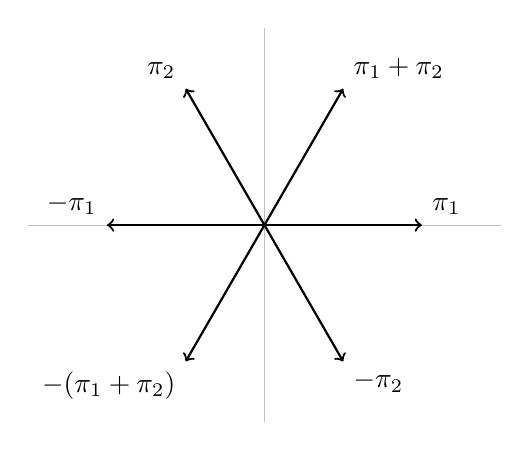
\begin{tikzpicture}[scale=2]
\draw[thin,lightgray] (-1.5,0) -- (1.5,0);
\draw[thin,lightgray] (0,-1.25) -- (0,1.25);
\draw[thick,->] (0,0) -- (1,0) node[above right] {$\pi_1$};
\draw[thick,->] (0,0) -- (cos 120,sin 120) node[above left] {$\pi_2$};
\draw[thick,->] (0,0) -- (-1,0) node[above left] {$-\pi_1$};
\draw[thick,->] (0,0) -- (-cos 120,-sin 120) node[below right] {$-\pi_2$};
\draw[thick,->] (0,0) -- (cos 60,sin 60) node[above right] {$\pi_1+\pi_2$};
\draw[thick,->] (0,0) -- (-cos 60,-sin 60) node[below left] {$-(\pi_1+\pi_2)$};
\end{tikzpicture}
\end{center}
Since $H^*=\lspan_\C(\Pi)$, we have $\dim H^*=2$, thus the dimension of the Cartan  subalgebra is also $2$. Since $|\Phi|=6$, we know that any Cartan-Weyl basis of the Lie algebra $A_2$ must have $2+6=8$ elements. Hence, the dimension of $A_2$ is 8. 

To complete our reconstruction of $A_2$, we would now like to understand how its bracket behaves. This amounts to finding its structure constants. Note that since $\dim A_2 = 8$, the structure constants $C^k_{\phantom{h}ij}$ consist of $8^3=512$ complex numbers (not all unrelated, of course).

Denote by $\{h_1,h_2,e_3,\ldots,e_8\}$ a Cartan-Weyl basis of $A_2$, so that $H=\lspan_\C(\{h_1,h_2\})$ and the $e_\alpha$ are eigenvectors of every $h\in H$.
Since $A_2$ is simple, $H$ is abelian and hence
\bse
[h_1,h_2] = 0 \quad \Rightarrow \quad C^k_{\phantom{k}12}=C^k_{\phantom{k}21} = 0, \quad \forall \, 1\leq k \leq 8.
\ese
To each $e_\alpha$, for $3\leq \alpha \leq 8$, there is an associated $\lambda_\alpha\in\Phi$ such that
\bse
\forall \, h \in H : \ \ad(h)e_\alpha = \lambda_\alpha(h) e_\alpha.
\ese
In particular, for the basis elements $h_1,h_2$,
\bi{rCl}
[h_1,e_\alpha] & = & \ad(h_1)e_\alpha = \lambda_\alpha(h_1) e_\alpha,\\
{[h_2,e_\alpha]} & = & \ad(h_2)e_\alpha = \lambda_\alpha(h_2) e_\alpha,
\ei
so that we have
\bi{rCl}
C^1_{\phantom{1}1\alpha}=C^2_{\phantom{2}1\alpha}=0, &\quad & C^\alpha_{\phantom{\alpha}1\alpha} = \lambda_\alpha(h_1) , \quad \forall \, 3\leq \alpha \leq 8,\\
C^1_{\phantom{1}2\alpha}=C^2_{\phantom{2}2\alpha}=0, &\quad & C^\alpha_{\phantom{\alpha}2\alpha} = \lambda_\alpha(h_2) , \quad \forall \, 3\leq \alpha \leq 8.
\ei
Finally, we need to determine $[e_\alpha,e_\beta]$. By using the Jacobi identity, we have
\bi{rCl}
[h_i,[e_\alpha,e_\beta]] & = & - [e_\alpha,[e_\beta,h_i]] -[e_\beta,[h_i,e_\alpha]] \\
& = & - [e_\alpha,-\lambda_\beta(h_i)e_\beta] -[e_\beta,\lambda_\alpha(h_i)e_\alpha] \\
& = & \lambda_\beta(h_i) [e_\alpha,e_\beta] +\lambda_\alpha(h_i)[e_\alpha,e_\beta]\\
& = & (\lambda_\alpha(h_i)+\lambda_\beta(h_i) )[e_\alpha,e_\beta]  ,
\ei
that is,
\bse
\ad(h_i)[e_\alpha,e_\beta] =  (\lambda_\alpha(h_i)+\lambda_\beta(h_i) )[e_\alpha,e_\beta].
\ese

If $\lambda_\alpha+\lambda_\beta\in\Phi$, we have $[e_\alpha,e_\beta]=\xi e_\gamma$ for some $3\leq \gamma \leq 8$ and $\xi \in \C$. Let us label the roots in our previous plot as
\begin{center}
\def\arraystretch{1.25}
\setlength\tabcolsep{10pt}
\begin{tabular}{c|c|c|c|c|c}
$\lambda_3$ & $\lambda_4$ & $\lambda_5$ & $\lambda_6$ & $\lambda_7$ & $\lambda_8$\\
\hline
$\pi_1$ & $\pi_2$ & $\pi_1+\pi_2$ & $-\pi_1$ & $-\pi_2$ & $-(\pi_1+\pi_2)$ 
\end{tabular}
\end{center}
Then, for example
\bse
\ad(h)[e_3,e_4] = (\pi_1+\pi_2)(h) [e_3,e_4],
\ese
and hence $[e_3,e_4]$ is an eigenvector of $\ad(h)$ with eigenvalues $(\pi_1+\pi_2)(h)$. But so is $e_5$! Hence, we must have $[e_3,e_4]=\xi e_5$ for some $\xi \in \C$. Similarly, $[e_5,e_7]=\xi e_3$, and so on.

If $\lambda_\alpha+\lambda_\beta\notin\Phi$, then in order for the equation above to hold, we must have either $[e_\alpha,e_\beta]=0$ (so both sides are zero), or $\lambda_\alpha(h)+\lambda_\beta(h)=0$ for all $h$, i.e.\ $\lambda_\alpha+\lambda_\beta=0$ as a functional. In the latter case, we must have $[e_\alpha,e_\beta]\in H$. This follows from a stronger version of the maximality property of the Cartan subalgebra $H$ of a simple Lie algebra $L$, namely that
\bse
\big(\forall \, h \in H : [h,x] = 0 \big)  \Rightarrow x\in H.
\ese
Summarising, we have
\bse
[e_\alpha,e_\beta] =
\begin{cases}
\xi e_\gamma & \text{if } \lambda_\alpha+\lambda_\beta\in\Phi\\
\in H & \text{if } \lambda_\alpha+\lambda_\beta=0\\
0 & \text{otherwise }
\end{cases}
\ese
and these relations con be used to determine the remaining structure constants of $A_2$.

























